\documentclass[12pt]{article}

% Packages
\usepackage[a4paper, top=2.5cm, bottom=2.5cm, left=2.5cm, right=2.5cm]{geometry}
\usepackage[utf8]{inputenc}
\usepackage[T1]{fontenc}
\usepackage{lmodern}
\usepackage[magyar]{babel}
\usepackage{amsmath}
\usepackage{graphicx}
\usepackage[colorlinks = true, linkcolor=blue, urlcolor=blue]{hyperref}
\usepackage{subfigure}
\usepackage{enumitem}
\usepackage{xcolor}
\usepackage{amssymb}
\usepackage{tikz}
\usepackage{fancyhdr}
\usepackage[newfloat]{minted}
\usepackage{caption}
\usepackage{indentfirst}
\usepackage{tcolorbox}
\tcbuselibrary{breakable}
\usepackage{etoolbox}
\usepackage{lscape}
\usepackage{pdflscape}

% Commands
\renewcommand{\thepage}{-- \arabic{page} --}
\newcommand\pikture[4]{\begin{figure}[ht!]\centering\includegraphics[width=#4\linewidth]{pic/#1}\caption{#2}\label{#3}\end{figure}}

\newcommand{\say}[2]{%
	{\rule[0.5ex]{\linewidth}{0.5pt}\hskip-3em\raisebox{-0.4em}{
\begin{tikzpicture}[scale=0.008]
				\fill (48.656200,67.906197)..controls (48.656200,75.199203) and (43.636700,84.164101)..(26.421900,84.164101)
				..controls (13.507800,84.164101) and (6.457030,75.796898)..(6.457030,68.144501)
				..controls (6.457030,63.839802) and (9.683590,62.882801)..(11.476600,62.882801)
				..controls (13.507800,62.882801) and (16.378901,64.320297)..(16.378901,67.906197)
				..controls (16.378901,70.656197) and (14.347700,72.808601)..(11.359400,72.808601)
				..controls (10.640600,72.808601) and (10.402300,72.808601)..(10.160200,72.687500)
				..controls (12.793000,78.902298) and (19.726601,81.773399)..(26.062500,81.773399)
				..controls (39.570301,81.773399) and (39.570301,73.046898)..(39.570301,68.503899)
				..controls (39.570301,61.449200) and (37.417999,59.179699)..(35.386700,57.027302)
				..controls (27.257799,48.300800) and (24.628901,37.179699)..(24.628901,29.886700)
				--(24.628901,24.148399)..controls (24.628901,21.996099) and (24.628901,21.519501)..(25.941401,21.519501)
				..controls (27.257799,21.519501) and (27.257799,22.355499)..(27.257799,24.507799)
				--(27.257799,28.929701)..controls (27.257799,35.984402) and (30.128901,46.503899)..(42.203098,55.472698)
				..controls (45.550800,57.984402) and (48.656200,61.687500)..(48.656200,67.906197)
				--cycle;
				\fill (31.679701,5.859380)..controls (31.679701,8.964840) and (29.050800,11.597700)..(25.941401,11.597700)
				..controls (22.355499,11.597700) and (20.085899,8.726560)..(20.085899,5.859380)
				..controls (20.085899,2.269530) and (22.953100,0.000000)..(25.824200,0.000000)
				..controls (29.171900,0.000000) and (31.679701,2.628910)..(31.679701,5.859380)
				--cycle;
	\end{tikzpicture}}}%
	{\hskip0.5em\textit{#1}\vskip0.5em}%
	{\begin{minipage}{\dimexpr\textwidth-20pt}{\hspace{15pt} #2}\end{minipage}\vskip0.5em\rule[0.5ex]{\linewidth}{0.5pt}\vskip0.5em}
}

\BeforeBeginEnvironment{minted}{\begin{tcolorbox}}%
	\AfterEndEnvironment{minted}{\end{tcolorbox}}%
	
\newtcbox{\inlinebox}{
	on line,
	boxrule=1pt,
	arc=2pt,
	left=2pt,right=2pt,top=1pt,bottom=1pt
}

% Title
\title{Felhők hálózati szolgáltatásai laboratórium (BMEVITMMB11)\\\textbf{Vorleser\\OCR alkalmazás}}
\author{Kovács~Bertalan\\\textbf{RHDBLM}}

\begin{document}
	\maketitle
	\thispagestyle{empty}
	
\includegraphics[width=.9\linewidth]{pic/vorleser-logo-full}
	\begingroup
	\renewcommand\thefootnote{}
	\footnotetext{A fenti képet a Google Gemini -- Nano Banana 2 modellje generálta.}
	\endgroup
	\clearpage
	
	\pagestyle{fancy}
	\fancyhead[R]{\textbf{Vorleser -- OCR alkalmazás}}
	\fancyhead[L]{Kovács~Bertalan -- RHDBLM}
	
	\tableofcontents
	\clearpage
	
	\section{CI/CD környezet}
	
	Ez a fejezet a Vorleser programhoz készült CI/CD környezet konfigurálását és beállítását taglalja egy egyszerű, két komponensből álló, \href{https://www.python.org/}{Python} alapú, \href{https://flask.palletsprojects.com/en/stable/}{Flask} szolgáltatáson keresztül. A CI/CD rendszer a \href{https://git-scm.com/}{Git} alapú \href{https://github.com/}{GitHub} szolgáltatást használja verziókezelő és integrációs, az \href{https://github.com/okd-project/okd}{OKD}-t pedig telepítési és futtatási környezetnek. OKD implementációnak a \href{https://console.okd.fured.cloud.bme.hu/}{BME által futtatott} OKD rendszert választottam.

	\say{Miért OKD?}{Az OKD a natív Kubernetes fölé építve olyan fejlesztői (PaaS) funkciókat biztosít, mint az integrált CI/CD – amelynek köszönhetően a telepítési folyamatok könnyen triggerelhetők GitHubról, és a rendszer a forráskódból automatikusan le is buildeli a szükséges Docker image-eket –, valamint a beépített szoftveres útválasztás és a robusztus belső DNS alapú szolgáltatás-felfedezés. Ezek a funkciók kellenek igazán a lazán csatolt mikroszolgáltatások kommunikációjához.}
	\subsection{Projekt struktúra}
	
	A példában egy kétszintű Flask alkalmazást hoztam létre. A projekt könyvtárszerkezete a következő:
	
	\begin{minted}{text}
vorleser/
|-- backend/
|   |-- app.py
|   |-- requirements.txt
|   |-- Dockerfile
|-- frontend/
|   |-- app.py
|   |-- requirements.txt
|   |-- Dockerfile
|-- .github/workflows/OKD_deploy.yaml
	\end{minted}
	
	A projekt megtalálható a GitHubon: \url{https://github.com/berci9ke101/vorleser}, ez a repozitórium fogja a későbbi Vorleser OCR program verziókezelő rendszerét biztosítani, tehát ide fognak majd a későbbi fájlok is kerülni.
	
	\subsection{A verziókezelő rendszer struktúrájának elve}
	
	A mikroszolgáltatások elveit követve minden komponens saját könyvtárral és Dockerfile-al rendelkezik, minimalizálva a függőségeket és így elősegítve a könnyű hordozhatóságot. A példában az alábbi Dockerfile-t használtam mindkét komponensnél (backend és frontend):
	
	\begin{minted}{dockerfile}
FROM python:3.9-slim
WORKDIR /app
COPY requirements.txt .
RUN pip install --no-cache-dir -r requirements.txt
COPY . .
CMD ["python", "app.py"]
	\end{minted}
	
	A későbbi OCR alkalmazás struktúrája is ezeken az alapokon fog működni.
	
	\subsection{A Flask alkamazás bemutatása}
	A CI/CD pipeline bemutatásához egy egyszerű Flask alkalmazást hoztam létre, amiben a backend publikál egy szövegrészletet a \inlinebox{\texttt{/api/data}} útvonalán. Ezt a szöveget felhasználva a frontend megjeleníti a backend üzenetét. A forráskódok alább olvashatóak:
	
	\textbf{Backend:}
	\begin{minted}{python}
from flask import Flask, jsonify

app = Flask(__name__)
@app.route('/api/data')
def get_data():
    return jsonify(message="Hello World!")

if __name__ == '__main__':
    app.run(host='0.0.0.0', port=5000)
 	\end{minted}
 	
	\textbf{Frontend:}
 	\begin{minted}[breaklines]{python}
from flask import Flask
import requests
import os

app = Flask(__name__)
@app.route('/')
def index():
   try:
       response = requests.get(f"http://{os.getenv('BACKEND_URL')} :5000/api/data")
       data = response.json()
       return f"<h1>Backend says: {data['message']}</h1>"
    except Exception as e:
       return f"<h1>Error: {str(e)}</h1>"

if __name__ == '__main__':
    app.run(host='0.0.0.0', port=3000)
 	\end{minted}
 	
 	A frontend a \inlinebox{\texttt{BACKEND\_URL}} környezeti változón meghatározott néven keresztül éri el a backendet. Ezt később be is állítottam.
	
	\subsection{Az OKD erőforrások létrehozása}
	
	Miután bejelentkeztem a BME webes felületén az OKD konzolba, kimásoltam a bejelentkezési parancsomat, majd az OKD platformon az alábbi parancsokkal inicializáltam a projektet és a szolgáltatásokat:
	
	\begin{minted}{bash}
# Bejelentkezés az OKD parancssori alkalmazásába
oc login --token=<..> \
	--server=https://api.okd.fured.cloud.bme.hu:6443

# A projekt létrehozása
oc new-project vorleser

# A build-ek létrehozása GitHub forrásból, ügyelve a kontextusra
oc new-app https://github.com/berci9ke101/vorleser.git \
	--context-dir=/backend \
	--name=vorleser-backend \
	--strategy=docker

oc new-app https://github.com/berci9ke101/vorleser.git \
	--context-dir=/frontend \
	--name=vorleser-frontend \
	--strategy=docker

# Szolgáltatások helyezése a komponensek elé és a portjaik kinyitása
oc expose deployment/vorleser-backend --port=5000 --target-port=5000
oc expose deployment/vorleser-frontend --port=3000 --target-port=3000

# A frontend szolgáltatás kiengedése alapértelmezett tanúsítvánnyal
oc expose svc/vorleser-frontend
oc patch route vorleser-frontend \
	-p '{"spec":{"tls":{"termination":"edge"}}}'
	\end{minted}
	
	Az OKD lehetővé teszi, hogy a verziókezelő rendszerben az egyes szolgáltatáskomponensek külön könyvtárban helyezkedjenek el. Ekkor az egyes komponensek kontextusát, a verziókezelő rendszerben elhelyezkedő, elérési útvonaluk alapján be kell állítani a fentebb látott \inlinebox{\texttt{--context-dir=<..>}} kapcsoló segítségével.
	
	Az alkalmazás elérhetőségéhez szolgáltatásokat hoztam létre a komponensek elé és kiengedtem a frontendet a nyílt Internetre. Mivel a klaszter alapértelmezetten a HTTPS használatára kényszerít, így az alapértelmezett bejövő tanúsítványt kellett használnom, azaz be kellett állítani az \textit{Edge TLS termination}-t \cite{okd-edge-termination}.
	
	A frontendnek megadtam a fentebb már említett backend elérhetőségét környezeti változóként:
	
	\begin{minted}{bash}
oc set env deployment/vorleser-frontend BACKEND_URL=vorleser-backend
	\end{minted}
	
	\subsection{Folyamatos integráció}
	
	A folyamatos integrációt a GitHub Actions segítségével valósítottam meg. Minden \inlinebox{\texttt{main}} ágra történő push esemény automatikusan elindítja a kód szintaktikai ellenőrzését. Ahhoz, hogy az OKD értesüljön az új verzióról a GitHub action bejelentkezik a BME OKD szerverére és értesíti az új verzióról. Ezután az OKD elkezdi a Docker image-ek buildelését.
	
	Az autentikációhoz létre kell hozni egy \inlinebox{\texttt{serviceaccount}}-ot. Ennek a menetét az alábbi parancsokkal végeztem el\footnote{A szükséges parancsok a BME OKD üzemeltetője, Bodor András útmutatása alapján születtek.}:
	\begin{minted}{bash}
cat <<EOF | oc apply -f -
apiVersion: rbac.authorization.k8s.io/v1
kind: Role
metadata:
  name: custom-build-instantiator
  namespace: vorleser
rules:
- apiGroups: ["build.openshift.io"]
  resources: ["buildconfigs/instantiate"]
  verbs: ["create"]
EOF

oc create rolebinding github-trigger-strict-binding \
  --role=custom-build-instantiator \
  --serviceaccount=vorleser:github-trigger \
  -n vorleser

oc create sa github-trigger
oc create token github-trigger --duration=8760h
	\end{minted}
	A sikerességről a következő képek számolnak be:
	
	\pikture{oc-create-role.png}{A megfelelő role létrehozása.}{fig:oc-create-role}{0.8}
	\pikture{oc-secret.png}{A token létrehozása a rolehoz.}{fig:oc-secret}{0.8}
	
	A kapott tokent el kell tárolni a GitHub repozitóriumban az \inlinebox{\texttt{Action secrets}} fül alatt:
	\pikture{okd-secret.png}{A GitHub Actions token eltárolása.}{fig:okd-secret}{0.8}
	
	Maga az action az alábbi yaml fájl segítségével fut le \cite{redhat-action-login}:
	
	\begin{tcolorbox}[breakable]
	\inputminted[breaklines]{yaml}{./yaml.txt}
	\end{tcolorbox}
	
	Az action sikeres lefutása után már nézhetjük is az OKD webes felületén a, ahogy a komponenseink elindulnak:
	
	\pikture{gh-succ.png}{Sikeres GitHub Actions lefutás.}{fig:gh-succ}{0.8}
	
	\pikture{okd-build-in-progress.png}{Folyamatban lévő build-ek az OKD konzolon.}{fig:okdbuild}{0.6}
	
	Megtekintve a \url{https://vorleser-frontend-vorleser.apps.okd.fured.cloud.bme.hu/} linket láthatjuk, hogy működik az alkalmazás:
	
	\pikture{working.png}{A működő alkalmazás.}{fig:working}{0.8}
	
	\subsection{Összegzés}
	A jelen fejezetben bemutatott folyamat elsősorban a Vorleser alkalmazás alapjául szolgáló CI/CD környezet és az OKD platform képességeinek demonstrálására fókuszált. A felépített architektúra egy leegyszerűsített, kétkomponensű Flask alkalmazáson keresztül igazolta a GitHub Actions és az OKD integrációjának zökkenőmentes működését.
	
	Fontos megjegyezni, hogy ez az implementáció csupán egy kezdeti, \textit{``proof of concept''} fázis volt az alapvető telepítési folyamatok hitelesítésére. A végleges optikai karakterfelismerő (OCR) mikroszolgáltatás-rendszer bevezetésekor ez a bemutatott alap egy jóval kiforrottabb, ``kipolírozott'' CI/CD pipeline-ná fog bővülni. A végleges folyamat a kódminőség szigorúbb ellenőrzését, komplexebb tesztelési fázisokat és a mikroszolgáltatások egymástól független, finomhangolt frissítését is automatizálni fogja a stabil felhős üzemeltetés érdekében.
	
	\clearpage
	\section{Weboldal + OCR detektálás funkció}
	Ez a fejezet a Vorleser alkalmazás elosztott architektúráját és a fejlesztés során hozott technológiai döntéseket mutatja be. A rendszer egy mikroszolgáltatás-alapú ökoszisztémára épül, ahol az egyes funkciókat – mint a webes interfész (\textit{Papagei}), az OCR feldolgozás (\textit{Leseratte}) és a bináris adattárolás (\textit{Maulwurf}) – önálló, saját fejlesztésű, egymástól lazán csatolt konténerizált komponensek látják el. A fejezet részletezi az aszinkron feladatkezelést biztosító \href{https://www.rabbitmq.com/}{RabbitMQ} (\textit{Brieftaube}) üzenetsor integrációját, a \href{https://github.com/JaidedAI/EasyOCR}{EasyOCR} könyvtár alkalmazását, valamint a \href{https://www.postgresql.org/}{PostgreSQL} (\textit{Elefant}) alapú perzisztens adattárolást.
	
	\subsection{Projekt struktúra}
	A Vorleser alkalmazás jelenlegi struktúrája a következő (dokumentáció, licenszelés stb. elhagyásával):
	\begin{minted}{bash}
vorleser/
|-- .github/workflows/OKD_deploy.yaml # CI/CD pipeline leíró
|-- k8s/ # Deklaratív kubernetes leírók
|   |-- blob-storage-deployment.yaml
|   |-- blob-storage-pvc.yaml
|   |-- frontend-deployment.yaml
|   |-- ocr-worker-deployment.yaml
|   |-- postgres-deployment.yaml
|   |-- postgres-pvc.yaml
|   |-- rabbitmq-deplyoment.yaml
|-- leseratte/ # OCR Worker
|   |-- app.py
|   |-- requirements.txt
|   |-- Dockerfile
|-- maulwurf/ # Blob Storage
|   |-- app.py
|   |-- requirements.txt
|   |-- Dockerfile
|   |-- test_app.py
|-- papagei/ # Frontend & API Gateway
|   |-- templates/
|   |   |-- 404.html
|   |   |-- index.html
|   |   |-- view.html
|   |-- app.py
|   |-- requirements.txt
|   |-- Dockerfile
|-- docker-compose.yaml # Lokális teszteléshez
	\end{minted}
	
	A projekt megtalálható a GitHubon: \url{https://github.com/berci9ke101/vorleser}
	
	\subsection{Komponensek rövid bemutatása és technológia választások indoklása}
	\begin{itemize}
		\item \textbf{\textit{Papagei} (Frontend \& API Gateway):} A \textit{Papagei} nem csupán a webes alkalmazás, hanem egy átjáró, amely összefogja a \textit{Maulwurf} (tároló), az \textit{Elefant} (adatbázis) és a \textit{Brieftaube} (üzenetsor) hívásait. Konténerizáltam, hogy az OKD-ban egyszerűen publikálható és elérhető legyen kívülről.
		\item \textbf{\textit{Leseratte} (OCR feldolgozó):} Az OCR művelet (EasyOCR modellek betöltése és futtatása) lassú és számításigényes. Ha ez a frontendben futna, a felhasználói felület megállna. Ha megnő a feltöltött képek száma, példányszáma növelhető anélkül, hogy a frontendhez hozzá kellene nyúlni.
		
		\say{Miért nem FaaS?}{Bár az OCR feladat elméletileg alkalmas lenne FaaS (Function as a Service) megoldásra a párhuzamos végrehajtás miatt, a konténeres megoldást választottam, mert az EasyOCR modellek több gigabájtosak és betöltésük jelentős időt vesz igénybe, ami egy FaaS filozófiába nem illene bele.}
		\item \textbf{\textit{Maulwurf} (Blob tároló):} Ahelyett, hogy minden pod közvetlenül csatlakozna egy megosztott fájlrendszerhez, a \textit{Maulwurf} egy egységes API-t biztosít a szolgáltatásoknak a képek tárolására. Ez lehetővé teszi, hogy később a fájlrendszert akár S3-ra vagy más felhős tárolóra cseréljük. Egy PVC biztosítja a fájlok integritását egy újraindítást követően.
		\item \textbf{\textit{Elefant} (PostgreSQL adatbázis):} A képek metaadatait az \inlinebox{\texttt{images}} táblában (\inlinebox{\texttt{id}}, \inlinebox{\texttt{blob\_id}}, \inlinebox{\texttt{description}}, \inlinebox{\texttt{status}}, \inlinebox{\texttt{detected\_text}}) relációs formában tároljuk a konzisztencia miatt. A \inlinebox{\texttt{detected\_text}} oszlop \inlinebox{\texttt{JSONB}} típusa lehetővé teszi az OCR által talált szövegek és koordináták rugalmas, mégis strukturált tárolását. Egy PVC biztosítja az adatok integritását pod újraindítást követően is.
		\item \textbf{\textit{Brieftaube} (RabbitMQ üzenetsor):} A \textit{Papagei} (Frontend \& API Gateway) és a \textit{Leseratte} (OCR feldolgozó) közötti laza csatolást az \inlinebox{\texttt{ocr\_tasks}} nevű üzenetsor valósítja meg. Ez garantálja a feladatok megőrzését a feldolgozó egység túlterheltsége vagy elérhetetlensége esetén is, hiszen a feldolgozás közben megszakadt munkafolyamatok üzenetei automatikusan visszakerülnek a sorba az ismételt végrehajtáshoz.
	\end{itemize}
	
	\subsection{A komponensek kommunikációjának áttekintése}
	A rendszer belső adatforgalmát a mikroszolgáltatások közötti laza csatolás és a hibatűrő üzenetküldés jellemzi. Az \hyperref[fig:arch-overview]{alábbi} ábra az ökoszisztéma belső interakcióit és a folyamatok logikai sorrendjét mutatja be a kép feltöltésétől az eredmények megjelenítéséig.
	
	\begin{landscape}
		\begin{figure}[!t]
			\centering
			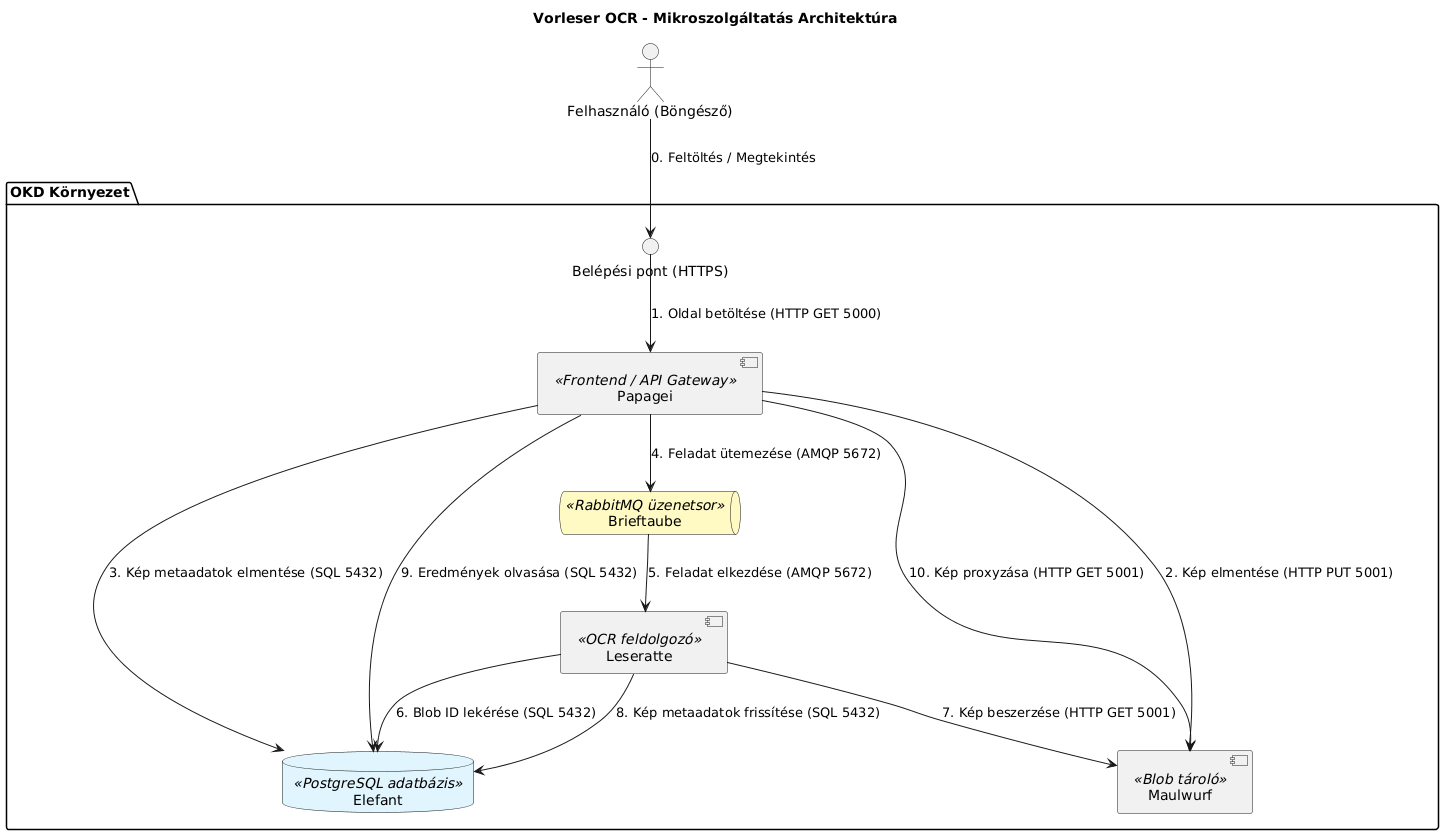
\includegraphics[height=0.7\textheight]{pic/arch-overview.png}
			\caption{A Vorleser architektúrájának áttekintése}
			\label{fig:arch-overview}
		\end{figure}
		A folyamat menete (ld.\ \ref{fig:arch-overview}.\ ábra): a felhasználó feltölti a képet (0.), amit a \textit{Papagei} fogad (1.), elment a \textit{Maulwurf} tárolóba (2.) és rögzít az \textit{Elefant} adatbázisban (3.). Ezután aszinkron feladatüzenetet küld a \textit{Brieftaube} üzenetsorba (4.) a feldolgozás megkezdéséhez.
		
		A \textit{Leseratte} worker kiveszi az üzenetet (5.), megszerzi a Blob ID-t (6.) és letölti a képet a tárolóból (7.), majd az EasyOCR motorral elvégzi a szövegfelismerést. Az eredményeket és a sikeres állapotot (8.) közvetlenül az \textit{Elefant} adatbázisba jegyzi vissza.
		
		Végül a felhasználó a \textit{Papagei} felületén keresztül megtekinti az eredményeket (9.). Ez az elosztott felépítés garantálja, hogy a feladatok a komponensek esetleges leállása esetén sem vesznek el.
	\end{landscape}
	
	\subsection{A fejlesztett komponensek felületes vizsgálata}
	\subsubsection{Maulwurf}
	Több meglévő Blob tároló implementációt is használhattam volna, de az egyik egyetemi tárgy keretén belül csináltam már egy kezdetleges Blob tárolót, amit kiegészítettem a házi feladathoz.
	
	Maga a szolgáltatás pofon egyszerű, egyetlen végpontot publikál, melyen a \inlinebox{\texttt{PUT}}, \inlinebox{\texttt{GET}} és \inlinebox{\texttt{DELETE}} \textit{HTTP} metódusokkal lehet műveleteket, adott azonosítójú fájlokon, végezni. Ezen azonosítók célszerűen \textit{UUID}k, mivel felhasználom a \textit{Papagei} lekérdezéseinél és így óhatatlanul kikerülnek az \textit{URL} mezőbe.
	
	A bináris tároló teszteléséhez a Flask keretrendszer beépített tesztelési támogatását használtam \cite{flask-testing}. A tesztelési folyamat során a \inlinebox{\texttt{tempfile}} modul segítségével ideiglenes könyvtárakat hoztam létre, így biztosítva, hogy a tesztek izolált környezetben fussanak, és ne módosítsák a tényleges perzisztens tárolót \cite{temp-testing}. Ezek a tesztek a CI/CD folyamat során is lefutnak.
	
	\subsubsection{Leseratte}
	A \textit{Leseratte} aszinkron worker a \textit{Brieftaube} feladatait dolgozza fel. Az OCR-modellek a Docker build során kerülnek a konténerbe a hálózati függetlenség érdekében \cite{easy-ocr-usage}. A 8080-as porton futó \inlinebox{\texttt{/health}} végpont jelzi a készenlétet (200) vagy az inicializálást (503). A folyamat során a worker a \textit{Maulwurf}-tól kért képet elemzi, az eredményt pedig az \textit{Elefant} adatbázisba menti.
	
	Az OCR feldolgozó egység az adatbázis-műveletekhez a \inlinebox{\texttt{psycopg2}} könyvtárat használja, amely hatékony interfészt biztosít a PostgreSQL eléréséhez \cite{psycopg}. A komponens Dockerfile-ja az EasyOCR hivatalos ajánlásai alapján készült, különös tekintettel a szükséges rendszerfüggőségekre (pl. \inlinebox{\texttt{libgl1-mesa-dev}}) \cite{easy-ocr-docker}. A konténerizált környezetben a \inlinebox{\texttt{PYTHONUNBUFFERED=1}} környezeti változó beállítása biztosítja, hogy az alkalmazás naplói azonnal megjelenjenek a standard kimeneten, megkönnyítve a hibakeresést az OKD konzolján \cite{pythonbuffered}.
	
	\subsubsection{Papagei}
	A \textit{Papagei} a Vorleser alkalmazás központi belépési pontja és API átjárója, amely a felhasználói felület kiszolgálásáért és a mikroszolgáltatások közötti koordinációért felel. A szolgáltatás kezeli a képek feltöltését, továbbítja a bináris adatokat a \textit{Maulwurf} tárolóba, rögzíti a kezdeti metaadatokat az \textit{Elefant} adatbázisban, majd aszinkron feladatot ütemez a \textit{Brieftaube} üzenetsorba. Emellett egy belső proxy-t is biztosít, amely lehetővé teszi a tárolt képek megjelenítését\footnote{A proxy-ra a \textit{CORS} (Cross-Origin Resource Sharing) korlátozások elkerülése miatt van szükség, mivel a bináris adatok egy szeparált belső mikroszolgáltatáson helyezkednek el.}.
	
	A frontend a Flask sablonkezelő rendszerét alkalmazza a dinamikus HTML tartalom előállításához \cite{flask-templates}. A felismert szövegek vizuális megjelenítésekor a rendszer abszolút pozicionált \inlinebox{\texttt{div}} elemeket hoz létre rétegként az eredeti kép felett. Ez a megoldás nem csak a találatok bekeretezését teszi lehetővé, hanem a felhasználó közvetlenül ki is jelölheti és másolhatja a képen látható szöveget.
	
	\subsection{A CI/CD folyamat áttekintése}
	A Vorleser projekt folyamatos integrációját egy összetett GitHub Actions munkafolyamat automatizálja, amely minden \inlinebox{\texttt{main}} ágra történő feltöltéskor (\textit{push}) aktiválódik. A folyamat két fő szakaszra tagolódik: ellenőrzés és tesztelés, valamint az OKD alapú telepítés.
	
	A munkafolyamat első szakaszában a kódminőség biztosítása érdekében elkészítettem egy \textbf{lint} és egy \textbf{test} fázist, amely a \inlinebox{\texttt{pylint}} és a \inlinebox{\texttt{python-unittest}} segítségével ellenőrzi az implementált három mikroszolgáltatás szintaktikai és stilisztikai megfelelőségét, valamint elvégzi a tesztelésüket.
	
	A második szakaszban indul el a \textbf{deploy} fázis, amely az ellenőrzött kódból elkészíti a Docker képfájlokat, létrehozza a megfelelő erőforrásokat az OKD környezetben (\inlinebox{\texttt{PVC}}, \inlinebox{\texttt{service}}, \inlinebox{\texttt{route}}, \inlinebox{\texttt{deployment}}), valamint elindítja a megfelelő konténereket.
	
	Mivel a Kubernetes alapértelmezetten nem tartalmaz a Docker Compose \inlinebox{\texttt{depends\_on}} paraméteréhez hasonló függőségkezelést, a szolgáltatások indulási sorrendjét \textit{initContainer}-ekkel szabályzom \cite{k8s-dependencies}. Ezek a segédkonténerek hálózati ellenőrzésekkel (ebben a projektben leginkább \inlinebox{\texttt{nc -z}} parancsokkal) várakoznak az adatbázis és az üzenetsor elérhetőségére, mielőtt a fő alkalmazás elindulna.
	
	\subsection{Az RBAC hiba elhárítása}
	A telepítési folyamat során jogosultsági problémák merültek fel az OKD klaszteren, mivel a CI/CD triggert végző fióknak nem volt elegendő joga a \inlinebox{\texttt{PVC}}-k kezeléséhez. A hiba elhárításához a \inlinebox{\texttt{github-trigger}} service account-hoz hozzárendeltem az \inlinebox{\texttt{edit}} szerepkört a projekt névterében. A módosítás után a \inlinebox{\texttt{oc describe rolebinding edit}} parancs igazolta, hogy a jogosultságok megfelelően frissültek.
	
	\begin{minted}{bash}
# Az edit role hozzárendelése a service account-hoz
oc adm policy add-role-to-user edit \
system:serviceaccount:vorleser:github-trigger -n vorleser

# A beállítás ellenőrzése
oc get rolebindings -n vorleser

Name:         edit
Role:
  Kind:  ClusterRole
  Name:  edit
Subjects:
  Kind            Name            Namespace
  ----            ----            ---------
  ServiceAccount  github-trigger  vorleser
	\end{minted}
	
	\subsection{A működés bemutatása}
	Ahhoz, hogy elérjem az újonnan elkészített szolgáltatás lekértem a publikus címét az OKD-től:
	\begin{minted}{bash}
# Külső route elkérése
oc get route vorleser-papagei

NAME             HOST/PORT                                            
vorleser-pap..   vorleser-papagei-vorleser.apps.okd.fured.cloud.bme.hu
	\end{minted}
	
	Ezek után meglátogattam a \url{https://vorleser-papagei-vorleser.apps.okd.fured.cloud.bme.hu/} oldalt és feltöltöttem egy képet, illetve adtam leírást a képnek (ld.\ \ref{fig:web-upload}.\ ábra). Ezek után megtekintettem az analizált képet (ld.\ \ref{fig:web-analysis}.\ ábra).
	
	\pikture{web-upload.png}{A feltöltés menete.}{fig:web-upload}{0.3}
	
	\pikture{web-analysis.png}{A kész kép oldala.}{fig:web-analysis}{0.5}
	
	A beolvasott kép bármikor megtekinthető a \url{https://vorleser-papagei-vorleser.apps.okd.fured.cloud.bme.hu/view/c93b3a4e-0c7e-4210-bb41-5652c5dc6eb9_adatb.webp} oldalon.
	
	\clearpage
	\bibliographystyle{ieeetr}\phantomsection\addcontentsline{toc}{section}{\refname}\bibliography{bibliography}
	
\end{document}